% SVN info for this file
\svnidlong
{$HeadURL$}
{$LastChangedDate$}
{$LastChangedRevision$}
{$LastChangedBy$}

\chapter{Brevi cenni di teoria degli insiemi}
\labelAppendix{settheory}
\addtocontents{define}{\noindent\textls{\textsc{\textcolor{reddo}{Appendice B:}
\nowtitle}}
}{}
\addtocontents{theorema}{\noindent\textls{\textsc{\textcolor{reddo}{Appendice B:}
			\nowtitle}}
}{}
\begin{introduction}
‘‘Le note a piè di pagina sono le superfici ingannatrici che permettono ai paragrafi tentacolari di aderire alla realtà più ampia della biblioteca.''
\begin{flushright}
	\textsc{Nicholson Baker,} bibliotecario di Cthulhu.
\end{flushright}
\end{introduction}
% TO DO: cit
\lettrine[findent=1pt, nindent=0pt]{Q}{uando} nella vita di tutti i giorni utilizziamo i numeri naturali, lo facciamo con due scopi ben precisi:\\
\begin{itemize}
	\item \textbf{Contare} quanti oggetti ci sono in un insieme, associando una \textit{dimensione} ad esso: ‘‘Ci sono \textit{tre} mele nel cestino''.
	\item \textbf{Ordinare} un insieme di oggetti, ossia formare una sequenza assegnando un \textit{indice} ad ogni elemento dell'insieme: ‘‘Torino è la \textit{quarta} città italiana per numero di abitanti''.
\end{itemize}
\noindent Per insiemi \textit{finiti}, non c'è apparente differenza tra i due concetti. Osserviamo che il numero di naturali (compreso lo zero) prima della $n$-esima posizione sono $n$, dunque in una sequenza di elementi indicizzata da $0$ con ultimo indice $n$ si hanno $n+1$ elementi. In altre parole, ordinando gli elementi è possibile sapere quanti sono e viceversa.\\
Questa due nozioni, come vedremo, divergono non appena generalizziamo i due concetti di ‘‘contare'' e ‘‘ordinare'' agli insiemi infiniti: ci sono molteplici ordinali infiniti che corrispondono allo stesso cardinale; inoltre, sotto certe ipotesi, potrebbero esserci insiemi che ammettono cardinalità ma che \textit{non} ammettono ordinali!\\
Lo scopo di questo capitolo aggiuntivo è cercare di dare alcune basi di \textbf{teoria degli insiemi} e \textbf{teoria degli ordini}, con il preciso scopo di spiegare come si ‘‘conta'' e si ‘‘ordina'' su insiemi infiniti.\\
Dopo una premessa sugli \textit{assiomi} sui quali baseremo i nostri ragionamenti, partiremo dal definire \textit{insiemi (ben) ordinati}, necessari per introdurre gli \textit{ordinali} (finiti e infiniti); arriveremo a parlare dell'\textit{induzione transfinita}.\\
Successivamente, passeremo ai concetti di \textit{cardinalità} e \textit{numeri cardinali}, mostrando diverse proprietà (compreso lo stretto legame che li lega agli ordinali), concludendo con alcuni importanti teoremi e congetture.\\
Per maggiori approfondimenti rimandiamo a XXX e XXX.
\section{Teoria degli insiemi di Zermelo-Fraenkel e Assioma di Scelta}
% TO DO: add axiom environment
% TO DO: add proprietà environment
\section{Relazioni d'ordine parziale e buon ordine}
\begin{define}[Relazione d'ordine parziale [(debole)] e totale.]~{}\\
	Una relazione binaria $\leq$ su un insieme $P$ è un \textbf{ordine parziale (debole)}\index{ordine!parziale} di $P$ se è
	\begin{enumerate}
		\item \textbf{Riflessiva:} $p\leq p,\ \forall p\in P$.
		\item \textbf{Transitiva:} se $p\leq q$ e $q\leq r$, allora $p\leq r$.
	\end{enumerate}
	La coppia $\left(P,\leq\right)$ viene detta \textbf{insieme parzialmente ordinato}.\\
	Un ordine parziale è \textbf{totale}\index{ordine!parziale!totale} se vale anche
	\begin{enumerate}
		\setcounter{enumi}{3}
		\item \textbf{Confrontabilità:} $p\leq q$ o $q\leq p,\ \forall p,q\in P$.
	\end{enumerate}
\end{define}
\begin{define}[Relazione d'ordine parziale  {(forte)} e totale.]~{}\\
	Una relazione binaria $<$ su un insieme $P$ è un \textbf{ordine parziale forte}\index{ordine!parziale!forte} di $P$ se è
	\begin{enumerate}
		\item \textbf{Irriflessiva:} $p\nless p,\ \forall p\in P$.
		\item \textbf{Transitiva:} se $p<q$ e $q<r$, allora $p<r$.
	\end{enumerate}
	La coppia $\left(P,<\right)$ viene detta \textbf{insieme parzialmente ordinato}.\\
	Un ordine parziale forte è \textbf{totale} se vale anche
	\begin{enumerate}
		\setcounter{enumi}{3}
		\item \textbf{Confrontabilità:} $p<q$ o $p=q$ o $q<p,\ \forall p,q\in P$.
	\end{enumerate}
\end{define}
% Cercato di adattare il paragrafo index in https://math.stackexchange.com/questions/1860938/definition-of-ordinals-in-set-theory-in-layman-terms
Abbiamo detto che i naturali, come \textit{ordinali}, servono per ordine un insieme in una sequenza; dobbiamo capire, almeno intuitivamente, cosa intendiamo per \textit{sequenza}.\\
Una \textbf{sequenza} può essere immaginata come una lista di elementi in cui l'ordine di tali elementi è importante e la posizione di un certo elemento nella lista è determinato dalle posizioni degli elementi precedenti.\\
Prtanto, preso un generico insieme $X$, una \textbf{sequenza} deve essere una funzioneda un insieme totalmente ordinato $I$, detto \textit{insieme degli indici}, che ad ogni indice $i\in I$ associa un elemento di $X$.
\begin{equation*}
	\funztot{x}{\left(I,<\right)}{X}{i}{x(i)=x_i}
\end{equation*}
\begin{center}
		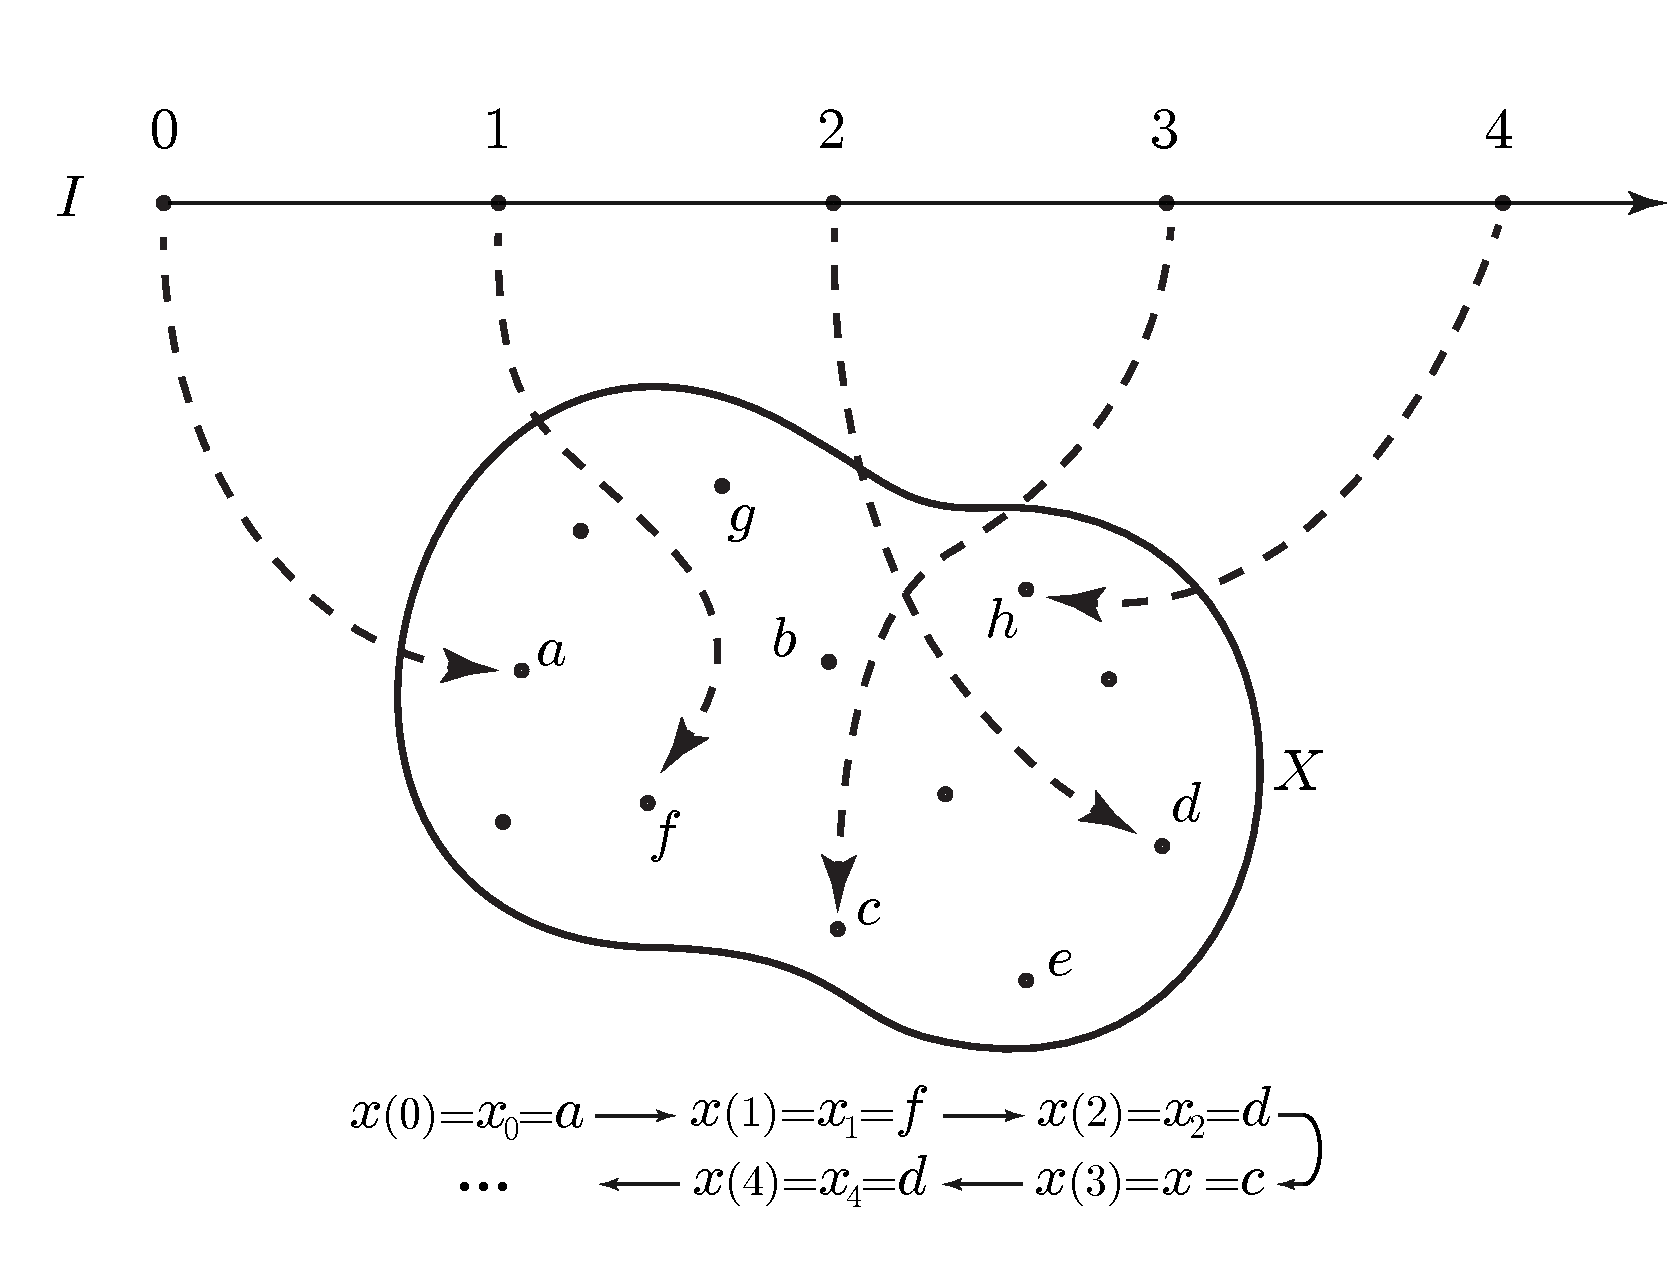
\includegraphics[trim=0cm 0cm 0cm 0cm, clip, scale=0.5]{images/settheorygrafico1.pdf}
\end{center}
È fondamentale che ci sia un \textbf{ordine} su $I$, dato che si vuole confrontare la \textit{posizione} di due elementi della sequenza: un elemento $x_i$ \textit{precede} un altro $x_j$ nella sequenza se gli indici sono tali per cui $i<j$.\\
Per soddisfare la seconda richiesta, ossia che la posizione di un certo elemento nella lista è determinato dalle posizioni degli elementi precedenti, si può pensare di definire la sequenza in modo \textit{ricorsiva}.
Tuttavia, per far ciò, \textit{non} è sufficiente che gli indici siano ordinati. Nello specifico, se $I$ contiene una \textit{sequenza infinita strettamente decrescente}, non siamo sicuri di poter definire ricorsivamente una successione a valori in $X$ indicizzata da $I$.\\
Invece, si può vedere che se $I$ \textit{non} ammette le sequenze infinite strettamente decrescenti, allora le definizioni ricorsive su $I$ sono lecite e permettono di definire univocamente una successione per ogni sequenza di indici! Dobbiamo quindi limitare quali relazioni d'ordine possiamo usare.
\begin{define}[Minimo.]~{}\\
	%[Massimali, minimali, estremi inferiori, superiori, massimi e minimi.]~{}\\
	Se $\left(P,\leq\right)$ è un insieme parzialmente ordinato, $X\neq\empty$ un sottoinsieme di $P$ e $a\in X$, allora:
	\begin{itemize}
		%\item $a$ è \textbf{massimale}\index{massimale} di $X$ se $a\in X$ e $\forall x\in X\ a\nless x$.
		%\item $a$ è \textbf{minimale}\index{minimale} di $X$ se $a\in X$ e $\forall x\in X\ x\nless a$.
		%\item $a$ è \textbf{massimo}\index{massimo} di $X$ se $a\in X$ e $\forall x\in X\ x\leq a$. Si indica $a=\max X$.
		\item $a$ è \textbf{minimo}\index{minimo} di $X$ se $a\in X$ e $\forall x\in X\ a\leq x$. Si indica $a=\min X$.
		%\item $a$ è \textbf{maggiorante}\index{maggiorante} di $X$ se $\forall x\in X\ x\leq a$.
		%\item $a$ è \textbf{minorante}\index{minorante} di $X$ se $\forall x\in X\ a\leq x$.
		%\item $a$ è \textbf{estremo superiore}\index{estremo!superiore} di $X$ se è il minimo dei maggioranti di $X$. Si indica $a=\sup X$.
		%\item $a$ è \textbf{estremo inferiore}\index{estremo!inferiore} di $X$ se è il massimo dei minoranti di $X$.  Si indica $a=\inf X$.
	\end{itemize}
\end{define}
\begin{define}[Buon ordine.]~{}\\
	Un ordine parziale totale $<$ di $P$ è un \textbf{buon ordine} se ogni sottoinsieme $X\neq \emptyset$ di $P$ ha un minimo.
\end{define}
\begin{examples}~{}
	\begin{itemize}
		\item $\naturalset$ è ben ordinato.
		\item $\integerset,\ \rationalset,\ \realset$ \textit{non} sono ben ordinati: tutti ammettono il sottoinsieme $\integerset_{<0}$ degli interi negativi, che non ha minimo.
	\end{itemize}
\end{examples}
\begin{observe}
	Ogni insieme ben ordinato \textit{non} ammette sequenze infinite strettamente decrescente, in quanto gli elementi della sequenza formano un sottoinsieme e pertanto esso ammette minimo.
\end{observe}
\begin{intuit}
	Possiamo ora capire perché non ha particolarmente senso definire successioni indicizzate, ad esempio, rispetto a $\left(\integerset,<\right)$ o rispetto a $\left(\realset,<\right)$: non ammettendo minimo, non possiamo avere il \textit{passo base} della nostra successione definita ricorsivamente!
\end{intuit}
\begin{digression}
	Il \textbf{teorema del buon ordine}, o anche noto come \textbf{teorema di Zermelo}, afferma che \textit{ogni} insieme non vuoto può essere ben ordinato (rispetto ad un opportuno ordine). Questo teorema risulta essere vero se si considera valido l'Assioma della Scelta; in realtà, si può ulteriormente mostrare come il teorema del buon ordine risulta essere equivalente, sotto gli Assiomi di Zermelo–Fraenkel, proprio all'Assioma della Scelta!
\end{digression}
\section{Ordinali}
L'idea ora è di definire gli \textit{ordinali} sulla base degli ordinali che lo precedono; infatti, ciò generalizza % TO DO: completare discorso
% TO DO: Jech, 2.19
Innanzitutto, diamo una definizione formale dei naturali come una famiglia di particolari insiemi costruiti \textit{ricorsivamente dall'insieme vuoto}.
\begin{define}[Numeri naturali.]~{}\\
	I \textbf{numeri naturali} $0,1,2,\ldots$ sono costruiti ricorsivamente nel seguente modo:
	\begin{equation}
		\begin{array}{l}
			0\coloneqq \emptyset\\
			n+1\coloneqq n\cup \left\{n\right\} = \left\{0,\ldots,n\right\}
		\end{array}
	\end{equation}
\end{define}
In altre parole:
\begin{equation*}
	\begin{array}{l}
		0=\left\{\emptyset\right\}\\
		1=\left\{0\right\}=\left\{\emptyset,\left\{\emptyset\right\}\right\}\\
		2=\left\{0,1\right\}=\left\{\emptyset,\left\{\emptyset\right\}, \left\{\emptyset,\left\{\emptyset\right\}\right\}\right\}\\
		\dots
	\end{array}
\end{equation*}
I naturali sono tutti degli insiemi \textit{ben ordinati}, identificabili dai seguenti diagrammi:
% TO DO: inserire diagrammi di Hesse
Poniamo allora il primo ordinale
\section{Cardinalità}
\begin{comment}
	Definiremo la cardinalità per insiemi \textit{ben ordinati}; poiché per l'\textit{Assioma di Scelta} ogni insieme è ben ordinato, la seguente definizione risulta essere valida sotto la teoria degli insiemi di \textbf{Zermelo–Fraenkel} con l'Assioma di Scelta ($\mathsf{ZFC}$).
\end{comment}
\begin{define}[Cardinalità.]~{}\\
	Due insiemi $X$ e $Y$ sono \textbf{equipotenti}\index{equipotenza} o \textbf{equinumerosi}\seeonlyindex{equinumerosità}{equipotenza}, in simboli
	\begin{equation}
		X\asymp Y
	\end{equation}
	se esiste una corrispondenza \textit{biunivoca} tra i due insiemi. L'equipotenza è una \textit{relazione di equivalenza} sulle classi di tutti gli insiemi; diciamo che due insiemi $X$ e $Y$ equipotenti hanno la stessa \textbf{cardinalità}\index{cardinalità} e lo indichiamo con
	\begin{equation}
		\abs{X}=\abs{Y}
	\end{equation}
\end{define}
\section{Cardinali}
\begin{comment}
	Ad ogni insieme $X$ possiamo assumere di associare il \textbf{numero cardinale}\seeonlyindex{numero!cardinale}{cardinalità} o \textbf{cardinale} $\abs{X}$, in modo tale che due insiemi che hanno lo stesso numero cardinale soddisfino la condizione di equipotenza.
	\begin{digression}
		Se consideriamo valido l'\textit{Assioma di Regolarità} è comunque possibile definire la cardinalità anche senza l'\textit{Assioma di Scelta} sulla base delle relazioni di equivalenza indotte dall'equipotenza.
	\end{digression}
	Ricordiamo che $X$ è \textit{finito} se è in corrispondenza biunivoca con un \textit{ordinale finito} $n\in\naturalset$:
	\begin{equation*}
		\abs{X}=\abs{n}
	\end{equation*}
	Poichè $\abs{n}=\abs{m}\iff n=m$, gli \textit{ordinali finiti} corrispondono ai \textit{cardinali finiti} e quindi $\abs{n}=n$, ossia
	\begin{equation*}
		\abs{X}=n
	\end{equation*}
	Denotiamo ora alcuni cardinali \textit{infiniti} che appaiono frequentemente:
	\begin{itemize}
		\item $\abs{\naturalset}=\aleph_{0}$: \textbf{cardinalità dei naturali}\index{cardinalità!dei naturali} o \textbf{cardinalità degli insiemi infinitamente numerabili} (si legge ‘‘\textit{aleph zero}'').
		\item $\abs{\realset}=\mathfrak{c}$: \textbf{cardinalità dei reali} o \textbf{cardinalità del continuo}\index{cardinalità!del continuo}.
	\end{itemize}
\end{comment}
\section{Ordine delle cardinalità}
\begin{define}[Iniezione.]~{}\\
	Un insieme $X$ si \textbf{inietta in} $Y$, in simboli 
	\begin{equation}
		X\precsim Y
	\end{equation}
	se esiste una funzione iniettiva $\funz{f}{X}{Y}$; in tal caso scriveremo
	\begin{equation}
		\abs{X}\leq\abs{Y}
	\end{equation}
\end{define}
La relazione $\precsim$ (o $\leq$ se ci riferiamo alle cardinalità) è una relazione d'\textit{ordine totale}: la relazione riflessiva e transitiva sono immediate, mentre l'antisimmetrica è garantita dal seguente teorema.
\begin{theorema}[Teorema di Cantor-Bernstein-Schröder.]~{}\\
	Se $\abs{X}\leq\abs{Y}$ e $\abs{Y}\leq\abs{X}$, allora $\abs{X}=\abs{Y}$.\\
	Equivalentemente, se esistono due funzioni \textit{iniettive}
	\begin{equation*}
		\funz{f}{X}{Y}\text{ e }\funz{g}{Y}{X}
	\end{equation*}
	allora esiste una funzione \textit{biettiva} $\funz{h}{X}{Y}$.
\end{theorema}
Un'altra conseguenza importante di questo teorema è quella di poter determinare la cardinalità sulla base di sole funzioni \textit{iniettive}.
\begin{examples}\textsc{Alcune applicazioni del teorema di Cantor-Bernstein-Schröder.}~{}
	\begin{itemize}
		\item L'intervallo $\left[0,1\right]$ ha la cardinalità del continuo; infatti, possiamo considerare le seguenti funzioni iniettive
		\begin{itemize}
			\item $\incl{\iota}{\left[0,1\right]}{\realset}$ inclusione.
			\item $\funztot{f}{\realset}{\left[0,1\right]}{x}{\frac{2\left(\arctan\left(x\right)+\frac{\pi}{2}\right)}{\pi}}$
		\end{itemize}
		\item Come visto a pag. XXX, dato l'insieme di Cantor $C$ si può definire una funzione $\funz{f}{C}{\left[0,1\right]}$ \textit{suriettiva}; in questo modo, $\abs{C}\geq \left[0,1\right]$ ma, in quanto $C\subseteq \left[0,1\right]$ si ha 
		\begin{equation*}
			\abs{C}=\left|\left[0,1\right]\right|=\mathfrak{c}
		\end{equation*} % TO DO: aggiunge pagina su Cantor o nelle note aggiuntive oppure nel libro in sè
	\end{itemize}
\end{examples}
Ci interessa anche definire una relazione d'\textit{ordine parziale forte} sulla base dell'iniezione precedentemente definita. 
\begin{define}[Iniezione stretta.]~{}\\
	Un insieme $X$ si \textbf{inietta strettamente in} $Y$, in simboli 
	\begin{equation}
		X\precnsim Y
	\end{equation}
	se esiste una funzione iniettiva $\funz{f}{X}{Y}$ ma non esistono funzioni suriettive $\funz{f}{X}{Y}$; in tal caso scriveremo
	\begin{equation}
		\abs{X}<\abs{Y}
	\end{equation}
\end{define}
\begin{observe}
	Si può vedere che
	\begin{equation}
		X \precnsim Y\iff X\precnsim Y\wedge X\asymp Y
	\end{equation}
	o, in termini di cardinalità,
	\begin{equation}
		\abs{X}<\abs{Y}\iff \abs{X}\leq \abs{Y}\wedge \abs{X}\neq\abs{Y}
	\end{equation}
\end{observe}


\begin{comment}
	Sulla base di queste definizioni possiamo enunciare già una serie di proprietà interessanti che collegano questa relazione d'ordine alle ben note \textit{relazioni insiemistiche} di inclusione e uguaglianza di insiemi.
	\begin{proposition}[Relazioni insiemistiche e ordine delle cardinalità.]~{}\\\label{cardinalitàugualenonimplicauguaglianzainsiemistica}
		Dati $X$ e $Y$ insiemi:
		\begin{itemize}
			\item $X\subseteq Y\iff \exists \incl{\iota}{X}{Y}$ inclusione $\iff \abs{X}\leq \abs{Y}$. %DUBBI sull'ultimo sse
			\item $X\supseteq Y\iff \exists \funz{f}{X}{Y}$ suriettiva $\iff \abs{X}\geq \abs{Y}$. % TO DO: controllare se è vero effettivamente
			\item Se $\abs{X}<\abs{Y}$, allora $X\subsetneqq Y$.
			\item Se $X$ e $Y$ sono \textit{finiti}, allora $\abs{X}=\abs{Y}\iff X=Y$; se $X$ e $Y$ sono \textit{infiniti} $\abs{X}=\abs{Y}\Ccancel[black]{\implies}X=Y$, ma vale soltanto la relazione banale $X=Y\implies \abs{X}=\abs{Y}$. % TO DO: aggiungere commento su questi risultati?
		\end{itemize}
	\end{proposition}
\end{comment}
\section{Aritmetica dei cardinali}
Possiamo definire delle \textit{operazioni aritmetiche} con i cardinali; dati $\abs{X}=\kappa$ e $\abs{Y}=\lambda$, si ha
\begin{align}
	\kappa+\lambda&=\abs{X\cup Y} \text{ se }X\text{ e }Y\text{ disgiunti}\\
	\kappa\cdot\lambda&=\abs{X\times Y}\\
	\kappa^{\lambda}&=\abs{X^Y}
\end{align}
dove con $X^Y$ indichiamo l'insieme delle funzioni da $Y$ in $X$.\\
Queste operazioni sono ben definite se sono indipendenti dalla scelta di $X$ e $Y$.
\section{Cardinalità dell'insieme delle parti}
\begin{theorema}[Biezione tra {$\setpart{X}$} e insieme delle funzioni da {$X$} in {$\{0,1\}$}.]~{}\\
	Dato un qualunque insieme $X$, sia $\setpart{X}$ l'insieme delle parti di $X$ e sia $2^X\coloneqq\left\{0,1\right\}^X$ l'insieme di tutte le funzioni $\funz{\ }{X}{\left\{0,1\right\}}$. Allora esiste una biezione tra $\setpart{X}$ e $2^X$, data da
	\begin{equation}
		\funztot{\Phi}{\setpart{X}}{2^X}{X}{\chi_X}
	\end{equation}
	con $\chi_X$ la \textit{funzione indicatrice} su $X$; l'inversa di tale funzione è la seguente:
	\begin{equation}
		\funztot{\Phi^{-1}}{2^X}{\setpart{X}}{f}{\left\{x\in\ X\mid f\left(x\right)=1\right\}}
	\end{equation}
\end{theorema}
\begin{corollary}[Cardinalità dell'insieme delle parti.]~{}\\
	Se un insieme $X$ ha cardinalità $\abs{X}$, l'insieme delle parti ha cardinalità
	\begin{equation}
		\abs{\setpart{X}}=2^{\abs{X}}
	\end{equation}
\end{corollary}
\begin{demonstration}
	Per il teorema precedente, si ha una biezione tra $\setpart{X}$ e $2^{\abs{X}}\coloneqq\left\{0,1\right\}^{X}$, dunque hanno la stessa cardinalità. Per esponenziazione dei cardinali, si ha
	\begin{equation*}
		\abs{\setpart{X}}=\left|\left\{0,1\right\}^{X}\right|=\left|\left\{0,1\right\}\right|^{\abs{X}}=2^{\abs{X}}
	\end{equation*}
\end{demonstration}
Poiché questo corollario vale sia per insiemi arbitrari, l'immediata conseguenza del corollario è poter definire la cardinalità dell'insieme delle parti di insiemi \textit{infiniti} già noti:
\begin{itemize}\label{cardinalitàinsiemepartiinfiniti}
	\item $\abs{\setpart{\naturalset}}=2^{\aleph_{0}}$
	\item $\abs{\setpart{\realset}}=2^{\mathfrak{c}}$
\end{itemize}
Il seguente teorema permette di dare di ordine \textit{non} triviale tra cardinali.
\begin{theorema}[Teorema di Cantor.]~{}\\
	Per ogni insieme $X$ si ha
	\begin{equation}
		X\precnsim\setpart{X}
	\end{equation}
	\begin{equation}
		\abs{X}<\abs{\setpart{X}}
	\end{equation}
\end{theorema}
\begin{demonstration}
	Sia per assurdo $\funz{f}{X}{\setpart{X}}$ una funzione suriettiva e sia
	\begin{equation*}
		Y=\left\{x\in X\mid x\notin f\left(x\right)\right\}
	\end{equation*}
	Per la suriettività di $f$ $\exists z\in X$ tale che $f\left(z\right)=Y$; tuttavia, si ha $z\in Y\iff z\notin f\left(z\right)=Y$, il che è assurdo. Segue che $X\nasymp\setpart{X}$.\\
	Invece, la funzione
	\begin{equation*}
		\funztot{f}{X}{\setpart{X}}{x}{\left\{x\right\}}
	\end{equation*}
	è iniettiva e quindi $X\precsim\setpart{X}$. Concludendo, $X\precnsim\setpart{X}$.
\end{demonstration}